\documentclass[coverpage]{inftechrep}
\usepackage{times}
\usepackage{graphicx}
\usepackage{algorithm}
\usepackage[noend]{algpseudocode}
\usepackage[nolist,nohyperlinks]{acronym}
\usepackage[numbers]{natbib}
\bibliographystyle{plain}

\begin{document}
\maintitle{Module}
\title{Coursework}
\author{Author}
\reportyear{2017}
\reportmonth{11}
\institutes{School of Informatics, University of Edinburgh}
\maketitle

\section{Introduction}
\label{sec:intro}

Victor recounts his fervent love for science, explaining, ``Curiosity, earnest research to learn the hidden laws of nature, gladness akin to rapture, as they were unfolded to me, are among the earliest sensations I can remember." \citep{shelley1994frankenstein}. A picture of his laboratory can be seen in Figure~\ref{fig:lab}.

\begin{figure}[h]
	\centering
	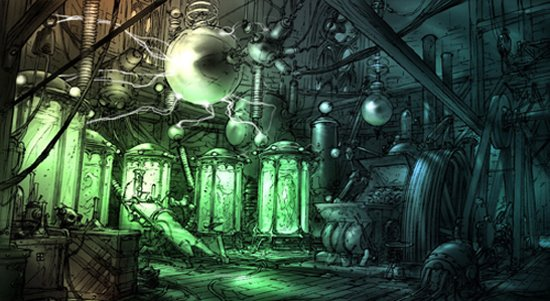
\includegraphics[width=6cm, height=4cm]{lab.jpg}
	\caption{Laboratory}
	\label{fig:lab}
\end{figure}

\section{Background}
\label{sec:back}

\section{Methodology}
\label{sec:method}

The following process will find the \ac{GCD}.

\begin{algorithm}
\caption{Euclid's Algorithm}\label{alg:euclid}
\begin{algorithmic}[1]
\Procedure{GCD }{$a,b$}
\State $r\gets a\bmod b$
\While{$r\not=0$}\Comment{only stop when r is zero}
\State $a\gets b$
\State $b\gets r$
\State $r\gets a\bmod b$
\EndWhile
\State \textbf{return} $b$\Comment{return gcd: b}
\EndProcedure
\end{algorithmic}
\end{algorithm}

\section{Results}
\label{sec:results}

\section{Discussion}
\label{sec:discuss}

\section{Conclusion}
\label{sec:conc}

\newpage
\bibliography{bibliography}

\begin{acronym}
	\acro{GCD}{Greatest Common Divisor}
\end{acronym}

\end{document}
